\documentclass[english]{beamer}
\usepackage[utf8]{inputenc}
\usepackage{amsmath,amssymb,amsfonts,amsthm}
\usepackage{graphicx}
\usepackage{fancyvrb}
\usepackage{float}
\usepackage{colortbl}
\usepackage{array}
\usepackage{lmodern}
\usepackage{multirow}
\usepackage{hhline}
\usepackage{picture}
\usepackage{subcaption}

\usepackage{pgfplots}

\pgfplotsset{compat=newest} % Allows to place the legend below plot
\usepgfplotslibrary{units} % Allows to enter the units nicely

\usepackage{rotating}

\setlength{\unitlength}{1cm}
\setlength{\parskip}{0.5\baselineskip}

%% ---------------------------------------------------------------------
%% COLOR DEFINITIONS

\definecolor{grisclair}{rgb}{0.9,0.9,0.9}
\definecolor{bluetitle}{rgb}{0.1,0.1,0.6}
\definecolor{tab}{rgb}{0.53,0.81,0.99}
\definecolor{red2}{rgb}{0.93,0,0}
\definecolor{red3}{rgb}{0.80,0,0}
\definecolor{bluev}{rgb}{0.2116,0.0104,0.7716} % BlueViolet
\definecolor{grey}{rgb}{  0.7505, 0.7826, 0.7793} % Gris
\definecolor{seagreen}{rgb}{0.2,0.5,0.5}
\definecolor{seagreen2}{rgb}{0.0000, 0.5676, 0.6179}
\definecolor{bluec}{rgb}{ 0.1999, 0.6294, 0.9597}
\definecolor{title2}{rgb}{0.2116, 0.0104, 0.7716}

%% foreground color shortcut commands
\newcommand{\black}[1]{\textcolor{black}{#1}}
\newcommand{\white}[1]{\textcolor{white}{#1}}
\newcommand{\yellow}[1]{\textcolor{yellow}{#1}}
\newcommand{\red}[1]{\textcolor{red3}{#1}}
\newcommand{\magenta}[1]{\textcolor{magenta}{#1}}
\newcommand{\bluet}[1]{\textcolor{bluetitle}{#1}}
\newcommand{\bluec}[1]{\textcolor{bluec}{#1}}
\newcommand{\bluev}[1]{\textcolor{bluev}{#1}}
\newcommand{\grey}[1]{\textcolor{grey}{#1}}
\newcommand{\cyan}[1]{\textcolor{cyan}{#1}}
\newcommand{\green}[1]{\textcolor{green}{#1}}
\newcommand{\sea}[1]{\textcolor{seagreen2}{#1}}
\newcommand{\seamii}[1]{\textcolor{seagreen}{#1}}

%% background color shortcut commands
\newcommand{\bgblack}[1]{\colorbox{black}{#1}}
\newcommand{\bgwhite}[1]{\colorbox{white}{#1}}
\newcommand{\bgyellow}[1]{\colorbox{yellow}{#1}}
\newcommand{\bgred}[1]{\colorbox{red}{#1}}
\newcommand{\bgmagenta}[1]{\colorbox{magenta}{#1}}
\newcommand{\bgblue}[1]{\colorbox{blue}{#1}}
\newcommand{\bgbluec}[1]{\colorbox{bluec}{#1}}
\newcommand{\bgbluev}[1]{\colorbox{bluev}{#1}}
\newcommand{\bggrey}[1]{\colorbox{grey}{#1}}
\newcommand{\bgcyan}[1]{\colorbox{cyan}{#1}}
\newcommand{\bggreen}[1]{\colorbox{green}{#1}}
\newcommand{\bggrisclair}[1]{\colorbox{grisclair}{#1}}

\hypersetup{colorlinks,linkcolor=,urlcolor=blue}

%% Beamer
\newcommand{\itemspace}{\vskip 5mm}
\newcommand{\itemtitle}[1]{darkblue{\textbf{#1}}}
\newcommand{\hl}[1]{\seamii{\textbf{#1}}}

\usepackage{sansmathaccent}
\pdfmapfile{+sansmathaccent.map}

\usecolortheme[named=bluetitle]{structure}
\beamertemplatenavigationsymbolsempty
\beamertemplatelargetitlepage

\useinnertheme[shadow]{rounded}

\setbeamercolor{section in head/foot}{fg=white!100}
\setbeamercolor{section in head/foot}{bg=bluetitle!80}
\setbeamercolor{section in head/foot shaded}{fg=white!100}
\setbeamercolor{section in head/foot shaded}{bg=bluetitle!80}

\setbeamertemplate{headline}
{
  \begin{beamercolorbox}{section in head/foot}
    \vskip1pt\insertsectionnavigationhorizontal{\paperwidth}{}{}\vskip1pt
  \end{beamercolorbox}%
}

\setbeamerfont{section in toc}{size=\large}
\setbeamerfont{section in toc}{series=\bfseries}
\setbeamercolor{section in toc}{fg=bluetitle}
\setbeamercolor{subsection in toc}{fg=bluetitle}
\setbeamertemplate{section in toc}[ball unnumbered]
\setbeamertemplate{subsection in toc}[ball unnumbered]

\setbeamertemplate{itemize item}[triangle]
\setbeamertemplate{itemize subitem}[ball]
\setbeamercolor{item}{fg=bluetitle!80}
\setbeamercolor{subitem}{fg=bluetitle!40}
\setbeamertemplate{mini frames}[box]

\useframetitletemplate{
  \centerline{\sea{\Large \textbf{\insertframetitle}}}
  \vskip -5mm
  \textcolor{black}{\hrule}
}

\usefoottemplate{%
  \vbox{
    \tinycolouredline{bluetitle!80}{\color{white}
      \hfill \insertframenumber~/~\inserttotalframenumber
    }
  }
}

\beamersetleftmargin{4mm}
\beamersetrightmargin{4mm}

\DeclareMathOperator*{\argmin}{arg\,min}

\title{
  FELICS-AE: a framework to benchmark lightweight authenticated block ciphers
}
\date{November 4\\2019}
\author{P. Huynh$^{(1)}$, K. Le Gouguec$^{(2)}$}
\institute{$^{(1)}$LORIA CNRS, $^{(2)}$Airbus CyberSecurity}


\AtBeginSection[]
{
  \begin{frame}<beamer>
    \tableofcontents[currentsection,subsectionstyle=show/show/shaded]
  \end{frame}
}


\begin{document}

\begin{frame}
  \titlepage
\end{frame}

\begin{frame}
  \tableofcontents
\end{frame}

\section[FELICS]{Background: the FELICS framework}

\begin{frame}
  \frametitle{The original FELICS framework}

  \url{https://www.cryptolux.org/index.php/FELICS}

  Benchmarking framework for crypto algorithms focused on small platforms

  \begin{itemize}
  \item Developed by the CryptoLUX research group at University of Luxembourg
  \item Focuses on block ciphers and stream ciphers
  \item Benchmark results showcased on the CryptoLUX wiki
  \end{itemize}

\end{frame}

\begin{frame}
  \frametitle{FELICS: platforms and metrics}

  \textbf{Platforms:}
  \begin{itemize}
  \item 8-bit AVR ATmega128 \emph{(simulated)}
  \item 16-bit MSP430F1611 \emph{(simulated)}
  \item 32-bit ARM Cortex-M3 \emph{(requires Arduino Due and J-Link probe)}
  \end{itemize}

  \pause

  \textbf{Metrics:}
  \begin{itemize}
  \item Binary code size
  \item RAM footprint
  \item Execution time
  \end{itemize}

\end{frame}

\section[FELICS-AE]{FELICS-AE additions}

\begin{frame}
  \frametitle{FELICS-AE}

  Started off FELICS v1.1.0 to compare \textsc{Lilliput-AE} to CAESAR's final lightweight portfolio (use-case 1)

  {\url{https://gitlab.inria.fr/minier/felics-ae}}
\end{frame}

\subsection{Support for \texttt{crypto\_aead}-compliant algorithms}

\begin{frame}
  \frametitle{\texttt{crypto\_aead}-compliant algorithms}

  Minimize work needed to add algorithms that comply with the API

  % For example, FELICS forbids some filenames to prevent clashes with framework plumbing (e.g. cipher.c, constants.h); we circumvented this by moving all FELICS headers into a dedicated felics folder (to "namespace" them) and renaming support files, so that integrators do not need to rename algorithm files.

  Not quite ``drop-in'' yet: still some idiosyncrasies from original FELICS

  \begin{itemize}
  \item \texttt{ROM\_DATA\_...}/\texttt{RAM\_DATA\_...} macros to specify alignment \& storage
  \item split files for encryption/decryption/common code
  \end{itemize}

\end{frame}

\subsection{New scripts to run benchmarks \& analyze results}

\begin{frame}
  \frametitle{\texttt{felics-run}}

  Orchestrates original FELICS entry points (scripts \& makefiles)

  Single output format (JSON) used by other scripts

\end{frame}

\begin{frame}[fragile]
  \frametitle{\texttt{felics-run} example}

\begin{Verbatim}[
  commandchars=\\\{\},
  codes={\catcode`\$=3},
  fontsize=\footnotesize
]
\$ ./scripts/felics-run -a PC Lilliput-II-128_vfelicsref
[...]
On PC
Lilliput-II-128 (felicsref, -O3): 6904 528 16792
\$ cat results/\$date-\$time-master.json
\{
    "commit": "ef3c770",
    "branch": "master",
    "data": [
        \{
            "cipher_name": "Lilliput-II-128",
            "architecture": "PC",
            "version": "felicsref",
            "compiler_options": "-O3",
            "code_size": 6904,
            "code_ram": 528,
            "code_time": 16792
        \}
    ]
\}
\end{Verbatim}

\end{frame}

\begin{frame}[fragile]
  \frametitle{\texttt{felics-compare}}

\begin{Verbatim}[
  commandchars=\\\{\},
  codes={\catcode`\$=3},
  fontsize=\footnotesize
]
\$ ./scripts/felics-compare old.json new.json
Comparing
	old.json
	(master) 1234567 Old commit summary
against
	new.json
	(master) 89abcde New commit summary

Lilliput-I-128 on AVR (vfelicsref with -Os)
	code_size: \textcolor{green}{-12.19%} (3166 $\searrow$ 2780)
	code_ram: \textcolor{green}{-49.22%} (514 $\searrow$ 261)
	code_time: \textcolor{red}{+32.05%} (189818 $\nearrow$ 250657)

Lilliput-I-192 on AVR (vfelicsref with -Os)
	code_size: \textcolor{green}{-10.47%} (3268 $\searrow$ 2926)
	code_ram: \textcolor{green}{-50.71%} (562 $\searrow$ 277)
	code_time: \textcolor{red}{+36.73%} (230309 $\nearrow$ 314893)
\end{Verbatim}

\end{frame}

\begin{frame}
  \frametitle{\texttt{felics-publish}}

  \texttt{\$ ./scripts/felics-publish foo.json -o foo.\$format}

  Options:

  \begin{description}
  \item[\texttt{-{}-sort-by}:] how setups are ordered
  \item[\texttt{-{}-filter}:] which setups are included
  \item[\texttt{-{}-info}:] which metadata and metrics are displayed
  \item[\texttt{-{}-table-label}:] anchor for documents supporting cross-references
  \item[\texttt{-{}-table-caption}:] additional text to describe the data set
  \end{description}

\end{frame}

\begin{frame}
  \frametitle{\texttt{felics-publish} examples}

  To \LaTeX:

  \begin{table}[H]
    \centering
    \tiny
    \begin{tabular}{l|l|l||r|r|r}
      \textbf{}                & \textbf{Version}   & \textbf{\texttt{CFLAGS}} & \textbf{Code size (B)} & \textbf{RAM (B)} & \textbf{Execution time (cycles)} \\ \hline
      \textsc{Lilliput-I-128}  & \texttt{felicsref} & \texttt{-O3}             &                   6100 &              266 &                           129093 \\ \hline
      \textsc{Lilliput-II-128} & \texttt{felicsref} & \texttt{-O3}             &                   6062 &              243 &                           132650 \\ \hline
      \textsc{Lilliput-I-128}  & \texttt{felicsref} & \texttt{-Os}             &                   2780 &              261 &                           250657 \\ \hline
      \textsc{Lilliput-II-128} & \texttt{felicsref} & \texttt{-Os}             &                   2768 &              229 &                           297992 \\ \hline
    \end{tabular}
    \caption{Performance results for 128-bit key algorithms on AVR ATmega128.}
    \label{table:bench-soft-128-avr}
  \end{table}

  % One table per architecture.

  To spreadsheet:

  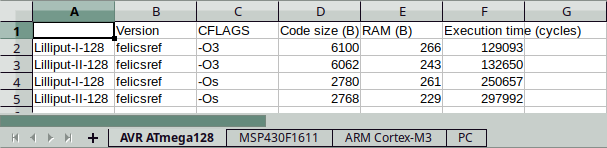
\includegraphics[width=\textwidth]{figures/felics-publish-ods.png}

  % One sheet (tab) per architecture.

\end{frame}

\subsection{Docker image}

\begin{frame}
  \frametitle{FELICS dependencies}

  Lots of dependencies to manage:

  \begin{table}[H]
    \centering
    \begin{tabular}{l|l|l}
      \textbf{Platform} & \textbf{Software} & \textbf{Origin}               \\
      \hline
      \multirow{2}{*}{AVR}
                        & simavr            & GitHub                        \\
                        & Avrora            & SourceForge + CryptoLUX patch \\
      \hline
      \multirow{2}{*}{MSP}
                        & MSP430-GCC        & Texas Instruments             \\
                        & MSPDebug          & GitHub                        \\
      \hline
      \multirow{1}{*}{ARM}
                        & J-Link Software   & SEGGER                        \\
      \hline
    \end{tabular}
    \caption{Extra-distro dependencies.}
    \label{table:dependencies}
  \end{table}

  How to distribute such a framework?

\end{frame}

\begin{frame}
  \frametitle{Distribution \& setup}

  Original FELICS solutions:

  \begin{itemize}
  \item Documentation\footnote{\url{https://www.cryptolux.org/index.php/FELICS_Prerequisites}}
  \item Virtual machine
  \end{itemize}

  \pause

  FELICS-AE additions:

  \begin{itemize}
  \item Script to fetch \& install all dependencies
  \item Scripts to generate \& run Docker image
  \end{itemize}

\end{frame}

\subsection{More platforms}

\begin{frame}
  \frametitle{New platforms}

  \textbf{Platforms:}
  \begin{itemize}
  \item 8-bit AVR ATmega128
  \item 16-bit MSP430F1611
  \item 32-bit ARM Cortex-M3
    \pause
  \item \bgyellow{NEW} 32-bit NRF52840 Cortex-M4
  \item \bgyellow{NEW} 32-bit STM32L053 Cortex-M0+
  \end{itemize}

\end{frame}

\section[Results]{Results with \textsc{Lilliput-AE}, \textsc{Ascon} and ACORN}

\begin{frame}
  \frametitle{Results}

  \url{https://paclido.fr/lilliput-ae/implementation/}

  \begin{itemize}
  \item \textsc{Lilliput-AE} on par with or faster than \textsc{Ascon} and ACORN on 8-bit and 16-bit
  \item much slower on 32-bit
  \end{itemize}

\end{frame}

\section[Future work]{Future work}

\begin{frame}
  \frametitle{Future work}

  \begin{itemize}
  \item Integrate more LWC candidates
  \item Support more than one test vector per algorithm
    % To make sure all branches are covered, e.g. with and without padding.
  \item Support more scenarios
    % The original FELICS scenarios have been removed (only 16B plaintext + 16B AD is supported right now).  felics-run could learn to set input sizes before compiling; this would be more versatile than having static scenarios with hardcoded input sizes.
  \item \texttt{documentation/TODO.md}
  \end{itemize}

\end{frame}

\section[Questions]{Questions}

\begin{frame}
  \frametitle{Any questions?}

  For more technical inquiries: \href{mailto:kevin.legouguec@airbus.com}{ask kevin.legouguec@airbus.com}!
\end{frame}

\end{document}
